%----------------------------------------------------------------
%
%  File    :  survey-intro.tex
%
%  Author  :  Keith Andrews, IICM, TU Graz, Austria
% 
%  Created :  27 May 1993
% 
%  Changed :  16 Nov 2010
% 
%----------------------------------------------------------------


\chapter{Web Tools For Accessibility Audits}

\label{chap:WebTools}



Web tools for accessibility audits provide core auditing functionality to anyone interested. The amount of tools in this category is large, where most of these tools come to the same conclusions for an audited web page regardless to the level of detail. This is due to several factors, one being that many of these web tools are using the same core library to assess the accessibility of a given web site. In the case of web accessibility, this library is called axe-core which is provided by the Deque company.

In this survey the tools that are inspected closely are but a fraction of the tools that are currently available on the web. The chosen tools were selected in a way, which enables a closer look at tools that run with the axe core library and without. Additionally the selection also tries to show the different qualities of each choice and what can be expected when someone tries to use these tools online.

In this survey our selection of web tools for accessibility audits consists of the following: Accessi, WAVE and Page Speed Insights which is the web tool equivalent to the Lighthouse browser extension. All of the mentioned web tools will be discussed in further detail in the following sections. For each of these three tools there were also videos created, which demonstrates the features and the functionality of each of the tools. The videos also give a quick overview of the metrics that were used to determine the accessibility of the tested web sites. 

\section{Accessi}

Accessi \parencite{Accessi} is one of the websites that were used to assess the accessibility of the two test pages. Accessi is a web site that offers a free accessibility test to its users. It works according to the Web Content Accessibility Guidelines (WCAG) standard. This can be further refined while using the tool by a choice of the 2.0 version of this standard or its in 2018 renewed 2.1 version.  
The web site will analyze the target test web site and give a basic rating in between 0-100\% telling the user basically the state of compliance of the test site. Through an automated test there are further metrics being detected, one example being a statistical analysis over the found issues of the web page. Accessi ranks these issues in three categorys: High impact, medium impact and low inpact. The high impact issues are the most obvious and intrusive ones, decending in severity, followed by medium and low. All the issues that are detected by the automated test run will additionally be listed, described and enhanced with examples. The feature that makes Accessi stand out from its competitors is the ability to export all of the aforementioned findings in PDF or csv format, giving the user a form of To-Do List or a fixed statement that they could work on if they would be looking towards improviong the accessibility of their web site. An example of the graphical interface of Accessi can be seen in Figure \ref{fig:accessi} below.

\begin{figure}[tp]
    \centering
    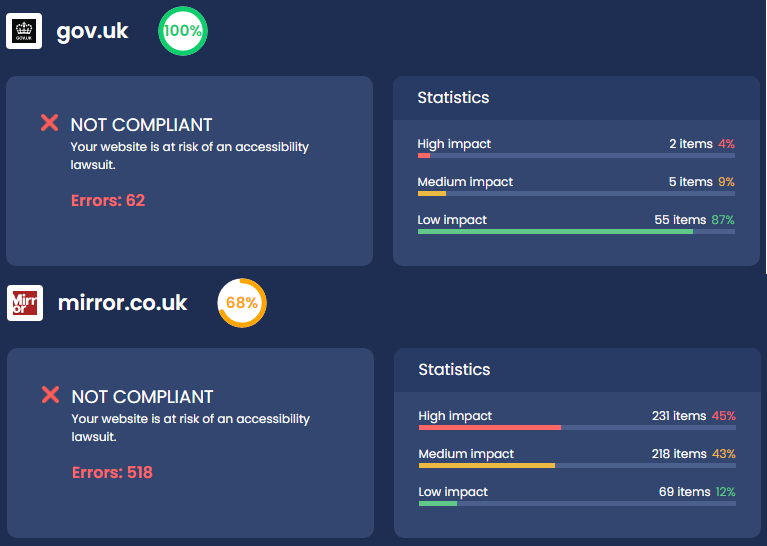
\includegraphics[keepaspectratio,width=\linewidth,height=\halfh]
    {images/accessi.png}
    
    \caption[Accessi Overview]
    {%
    Accessi web tool header showing an overview for each test site.
    }
    \label{fig:accessi}
\end{figure}

\section{WAVE}

WAVE \parencite{WAVE_web} is a tool provided by the company WebAim. As the tools described in this survey its purpose is to assess the accessibility of a website. WAVE offers a different take on the user interaction with a website which is subject to an accessibility test. The user is offered an interactive web tool, which embeds itself in the test website which is being surveyed. This embedded interface gives the user the ability to interactively inspect all the errors and warnings that are produced for a given website. The user is given the ability to click on icons which are attatched to elements of the test site, clearly outlining which element is considered non-compliant with accessibility guidelines. This interactivity is a special feature of the WAVE tool as through the course of research in our survey it is still the only tool providing these options. The interactive anture of the tool really provides the user with an indepth look into each error and where on the website it is located. In addition to this feature, WAVE also gives a summary over all the different kinds of errors or issues find on a given website.


\begin{figure}[tp]
    \centering
    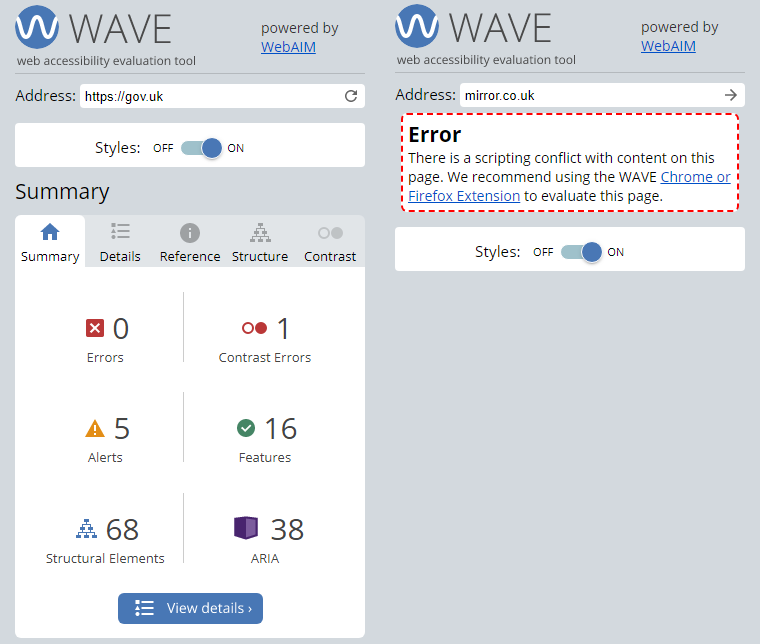
\includegraphics[keepaspectratio,width=\linewidth,height=\halfh]
    {images/WAVE.png}
    
    \caption[Accessi Overview]
    {%
    Accessi web tool header showing an overview for each test site.
    }
    \label{fig:accessi}
\end{figure}

\section{Page Speed Insights aka. Lighthouse}

Page Speed Insights \parencite{PSIL}
lorem ipsum


\section{Showcase videos}
In this survey two web sites were targeted for evaluation by the aforementioned tools. For a good expamle concerning web accessibility the \url{https://www.gov.uk/} web site was chosen where as for the negative example \url{https://www.mirror.co.uk/} was the choice. The videos that were produced each showcase the interaction between the user, the tools and the web site that is being evaluated respectively. A video of this format was produced for Accessi \parencite{Accessi_vid}, WAVE \parencite{WAVE_vid} and Page Speed Insights (Lighthouse) \parencite{PageSpeedInsights_vid}. All of these videos showcase the features of the tool that is being covered as well ass highlighting a few extras the tool of each video might have over other tools that might have a different focus. The outcome of all of the videos is yet the same, as they all evaluate the positive example as being very well rated and rating the negative example as being non-compliant with the usual standards of accessibility for web sites.

\section{Web Tools For Accesibility Audits Conclussion}

lorem ipsum


